% Setup - do not change
\documentclass[11pt]{article}
\usepackage[top=0.9in, left=0.9in, bottom=0.9in, right=0.9in]{geometry} 
\usepackage{parskip}

\usepackage[english]{babel}
\usepackage[utf8]{inputenc}
\usepackage{amsmath,amsthm,amssymb,graphicx,pdfpages,lipsum,hyperref}
\usepackage[none]{hyphenat}
\usepackage{csquotes}

\setlength\parindent{0pt}
%%%%%%%%%%%%%%%%%%%%%%%%%%%%%%%%%%%%%%%%%%%%%%%%%%%%%%%%%%%%%%%%%%%
% add other packages here if required
\graphicspath{ {plots/} }
\usepackage{wrapfig}
%% Bibliography is specified in this file. You can also choose an inline bib style if you want to. But make sure your citation style is consistent (and proper)
% For more details on citation: https://library.unimelb.edu.au/recite
\usepackage[sorting = none]{biblatex}
\addbibresource{references.bib}

%%%%%%%%%%%%%%%%%%%%%%%%%%%%%%%%%%%%%%%%%%%%%%%%%%%%%%%%%%%%%%%%%%% the '%' symbol denotes comments

% Begin document creation
% DELETE THE \lipsum PLACEHOLDERS WHEN YOU BEGIN
\title{\textbf{Earning Analysis for Yellow Taxi Drivers in NYC}}
\author{
Ziyi Li \\
Student ID: 1073869 \\
%% Replace the link with your GitHub repo
% 1. Remember to escape underscore (\_) in the link.
% 2. Remember to include the commit you want to submit in the link
\href{https://github.com/MAST30034-Applied-Data-Science/mast30034-project-1-LZY-Ziyi.git}{GitHub repo with commit}
}

\begin{document}
\maketitle

\section{Introduction}
% Link to a 30 min tutorial if you require revision: https://www.overleaf.com/learn/latex/Learn_LaTeX_in_30_minutes
% use \textbf{} for bold text and \textit{} for italic. 
% \texttt{} creates code blocks akin to `code ticks` in markdown
Taking a taxi has been an essential choice of travel mode for people to choose, therefore taxi driver would be a common job for citizens. This report focuses on analyzing the efficiency of earning for the yellow taxi drivers in New York City to support the taxi drivers to improve their income.

The main data set used by this report is TLC Trip Record Data, which is published by NYC Taxi \& Limousine Commission\cite{TLCdata}. The website provides data sets for different types of taxis including the yellow taxi, the green taxi, and the For-Hire Vehicle(FHV), I decided to research the yellow taxi because:1. Unlike the green taxi, the yellow taxi has the license to pick up passengers in any part of NYC. 2. Unlike the FHV, yellow taxis have clear and relatively complex rules for the fare that could be suitable to analyze. I use the data starting from January to March of the year 2022 since the latest data would be more valuable. Moreover, I want to analyze the impact of snow, while the snow for NYC mostly falls during the selected month. The initial data set has 9071244 records and 19 fields. The NYC TLC also provides the taxi zone data that helps us visualize the data geographically.

An external data set that describes the amount of daily snowfall in inches is published by Central New York's Live Weather\cite{2021-22snowFall} is used for the additional attributes. This data set starts recording the snowfall from July 2021 to Jun 2022, which covers all the dates we need to research.

I've named a new value called earning efficiency which is calculated by the total amount of earning of a trip divided by the time of the trip in minutes. I wish to use this to represent the efficiency of earning for every single trip. However earning within a single trip is not enough, the trip amount should also be considered to well define the earnings of the taxi drivers. Therefore, I studied the relationships of other features with the trip amount and earning efficiency. With the comparison of the two similar ordinary least squares linear models, related features are determined to give the final result.


% You can have \section{}, \subsection{}, and \subsubsection{}

\section{Data Preprocessing}
In this section, I will first show the processing steps of the data set, then analysis like the distribution of the attributes selected. After that, the relationship between these attributes and the target variable will also be studied. 

\subsection{Feature Selection}
The original taxi trip data set have 19 features, whereas some of them would be useless to analyze the earnings from the taxi driver's perspective. Features like Vendor ID that are clearly irrelevant to the earnings are directly discarded. While Features like drop-off location and passenger count that could not be decided by the taxi driver are also dropped. Fees like MTA tax, improvement surcharge, tolls amount, and congestion surcharge is assumed to be unrelated to drivers' income, therefore these fees and the total amount is also discarded. The remaining features are pickup date-time, drop-off date time, trip distance, pickup location ID, payment type, fare amount, extra fee, tip amount, and airport fee, these features are selected to be analyzing the income of the taxi driver. For the snowfall data set, the only data it contains is the date and snowfall amount, therefore all of the attributes are kept. After several data frame operations, the two data sets are merged by the date.

\subsection{Outlier Removing}
In order to get an overall concept, the minimum and the maximum of each attribute are checked. Various kinds of outliers are immediately found.

\begin{itemize} 
    \item Trip date outside the wanted range and invalid trip duration. For example, the earliest pickup time is in the year 2003, and some trips got drop-off time earlier than the pickup time. 8,522 observations are discarded for this situation.
    \item Trips start at the unknown location is defined that the Pickup location ID larger than 263, by checking the lookup table. 107,026 instances were removed.
    \item Trips with a trip distance less than roughly 100 meters (0.065 miles) are considered to be an outlier. Within this distance, walking might even be faster than waiting for a taxi. Surprisingly, 111,317 data are eliminated by this step.
    \item Trips with any unreasonable low fair including fare amount less than 2.5(the initial charge for the taxi trip), and any fee that is negative is illogical. After this 38,781 observations are removed.
    \item Payment type out of range or too small quantity for the payment type is also regarded as an outlier. 263,275 data for the type out of range and 32,821 data for the rare payment type. After the deletion, the payment type only remains for credit cards and cash.
    \item extremely large numerical data: for trip distance, fare amount, tip amount, and extra fee, Because all of these data are heavily right-skewed, in order not to lose too much information, data exceeding 6 times of interquartile range are regarded as outliers. 339,212 observations are removed.
\end{itemize} 
After the outlier removal, 8,170,290 instances are left.

\subsection{Missing Value Handling}
By checking the data, there are 291055 missing values for the airport fee attribute. By looking up the rule of taxi fare by NYC TLC, it is clearly stated that for taxis, there is a 1.25\$ airport fee for picking up at LaGuardia and John F. Kennedy Airports only. Therefore, I find the corresponding location id of these 2 airports and let the airport fee be 1.25\$ for the record which pick-up location ID fits these 2 locations and 0\$ for the rest to handle the missing value.

Moreover, the tip amount only collects the data from the trip paid by credit card. Assume the ratio of tip amount against the total fare (excluding tip amount) is the same no matter what payment type is. After summing up the fee columns as a new attribute, I compute this ratio for credit card payments and apply the ratio to the cash payment to get the tip amount for it. Afterward, the total payment is updated by summing up all the fee attributes including the tip amount. After getting the new total payment, these original fee features are no longer needed.

\subsection{Feature Engineering}
After the preprocessing steps, it's time to produce the attributes we aimed to analyze and the potential features that could influence it. The trip duration in seconds is simply calculated by using drop-off time minus pick-up time for each trip, then the duration is transformed into minutes. Since we already got the total payment for the trip, the earning efficiency could be computed by the total payment divided by the duration. Two new features 'times of day' which represent the hour of pick-up time of that day, and 'day of the week' which indicates the day in each week from Monday to Sunday are simply grabbed from the feature pick-up date time. While the numerical feature snowfall in inches didn't follow the normal distribution and can not take the log transform (the most data was 0 for snowfall), I decided to turn the snowfall into a feature that indicates whether the given day snowed or not.

Up until now, we have all the needed features. The date time data is no more needed, the payment data and the duration data are used to calculate the earning efficiency, we could not use them back to analyze the earning efficiency. The data we have now contains the numeric: attributes earning efficiency and trip distance; the categorical attributes: pick up location ID, time of day, day of the week, and snow or not.

\section{Data Analysis}
This section will focus on finding the distribution of numerical attributes and how all the other attributes are related to the earning efficiency and some with the trip amount.
\begin{figure}[h]

\begin{minipage}{.5\textwidth}
    \centering
    \caption{earning efficiency with 1000 bins} \label{f1}
    % change the scale multiplier to make the figures smaller or larger
    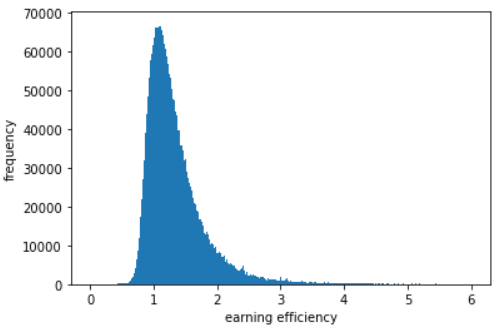
\includegraphics[width=1\textwidth]{earningHist.jpg}
\end{minipage}
\begin{minipage}{.5\textwidth}
    \centering
    \caption{new earning efficiency with 1000 bins} \label{f2}
    % change the scale multiplier to make the figures smaller or larger
    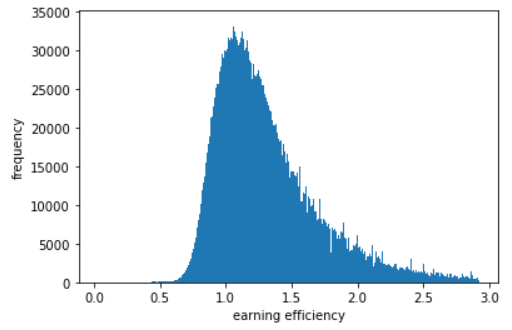
\includegraphics[width=1\textwidth]{earningHist2.jpg}
\end{minipage}
\end{figure}
\subsection{Earning Efficiency}
Due to the reason that the earning efficiency is the total fare divided by the duration, and there is an initial charge for every trip, the earning efficiency would become extremely high when the duration is very small. The mean of it is about 1.44, whereas the maximum of it reaches 3500. Therefore further outlier removing steps need to be performed. By plotting the distribution of earning efficiency with a range 0-6, see(Figure \ref{f1}), although the maximum value reaches 3500, most data are nearly normal distributed around the mode. I tried to use the 3$\sigma$
rule (we have nearly 99.73\% certainty that values are within 
$\mu\pm 3\sigma$ for a normal distribution) to remove the outlier but find that due to the extremely high values, the standard deviation goes pretty high, so I remove the earning efficiency with a value larger than 10, and then apply the $3\sigma$
rule to get rid of the outliers. The result distribution can be seen in (Figure \ref{f2}).

\subsection{Trip Distance}


\begin{wrapfigure}[13]{r}{23em} 
        \centering
        \caption{earning efficiency vs log trip distance} \label{f3}
        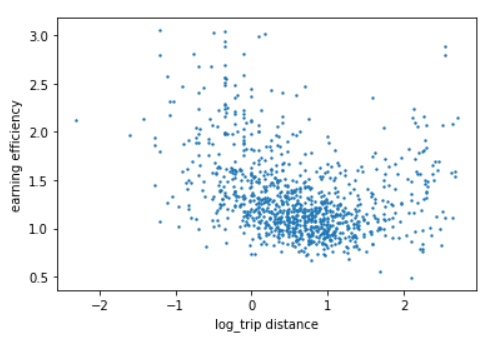
\includegraphics[width=0.5\textwidth]{plots/scatter.jpg}
\end{wrapfigure}
The distribution of trip distance as mentioned before is heavily right skewed, I decide to take a log transformation of it and it turns out to be roughly normally distributed. The scatter plot of earning efficiency vs log trip distance with 1000 samples (Figure \ref{f3}) shows that there could be a roughly negative linear relationship between the two variables. As the log trip distance exceeds 2, the earning efficiency seems to have an increasing trend, with could be a potential risk to fitting a linear model, I will try to fit the model and see what happens in the next section.

\subsection{Categorical Variables}
In order to find the relationship between earning efficiency and the categorical variables, I aggregated the earning efficiency with each categorical value separately and compute the mean of earning efficiency with each category. Moreover, the trip amount is also aggregated by each categorical value separately to get a sense of how likely a driver could get a trip order in a given time.
\subsubsection{Time of day}
Figure \ref{f4} shows That there is a strong relationship between two variables, where starting at 4 pm, the log earning efficiency keeps increasing until reach the second day's 5 am and reaches the peak. For the rest of day, the earning efficiency goes pretty low. The rule of taxi fare could be the reason for this: rush hour surcharge from 4 pm to 8 pm, and the overnight surcharge from 8 pm to 6 am. While Figure \ref{f5} clearly indicates that the trip amount goes to the peak at 6 pm, which is the center of rush hours, and the trip amount goes pretty low at the midnight.

\begin{figure}[h]

\begin{minipage}{.5\textwidth}
    \centering
    \caption{Mean earning efficiency in different time of day}\label{f4}
    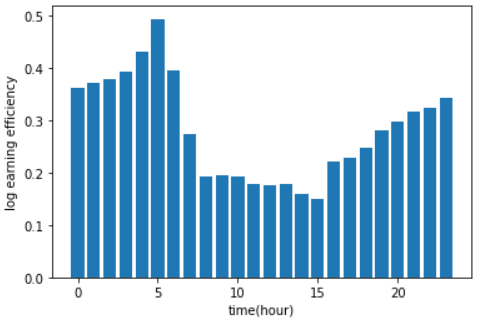
\includegraphics[width=0.95\textwidth]{earnTime.jpg}
\end{minipage}
\begin{minipage}{.5\textwidth}
    \centering
    \caption{Trip amount in different time of day} \label{f5}
    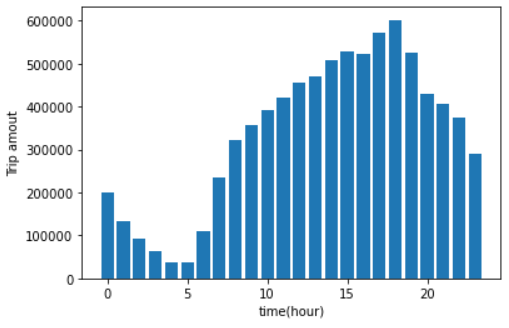
\includegraphics[width=1\textwidth]{plots/tripTime.jpg}
\end{minipage}
\end{figure}

\subsubsection{Day of Week}
Figure \ref{f6} clearly shows that the log earning efficiency goes down on Monday and reaches the bottom on Thursday, then starts to rise until Sunday and gets the highest log earning efficiency for a single trip, while Figure \ref{f7} tell us the trip amount got completely opposite relationship with the day of the week by comparing to the earning efficiency.

\begin{figure}[h]

\begin{minipage}{.5\textwidth}
    \centering
    \caption{Mean log earning efficiency on a different day of week}\label{f6}
    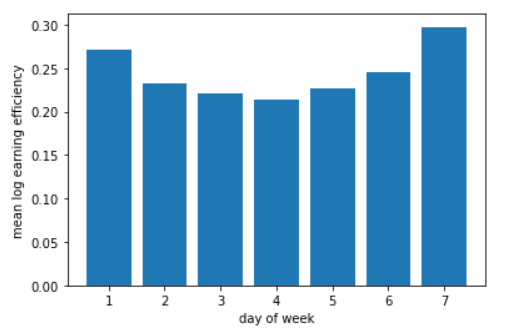
\includegraphics[width=0.95\textwidth]{plots/week1.jpg}
\end{minipage}
\begin{minipage}{.5\textwidth}
    \centering
    \caption{Trip amount in different day of week} \label{f7}
    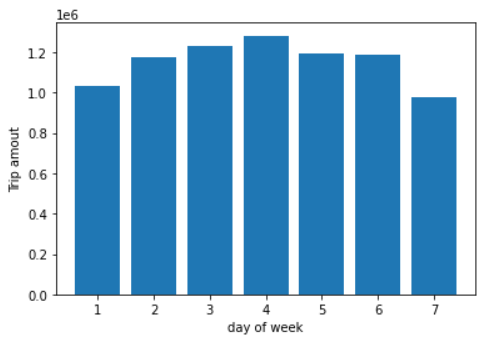
\includegraphics[width=0.95\textwidth]{week2.jpg}
\end{minipage}

\end{figure}
\subsubsection{Snow}
The snow attribute got the same aggregating operation with the log earning rate and the trip amount. The snowing weather got a 0.02 amount higher log earning rate than the weather without snow, while the average trip amount for snowing weather got a bit less than the non-snow weather.
\subsubsection{Geospatial Visualisation of Pick-up Location}

\begin{figure}[h]
\begin{minipage}{.5\textwidth}
    \centering
    \caption{Log Sum Earning Efficiency for Pick-up Location}\label{f8}
    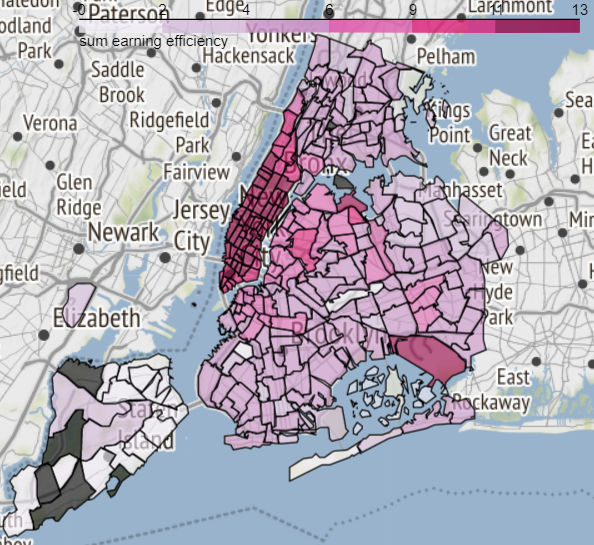
\includegraphics[width=0.95\textwidth]{geo1.jpg}
\end{minipage}
\begin{minipage}{.5\textwidth}
    \centering
    \caption{Mean Earning Efficiency for Pick-up Location} \label{f9}
    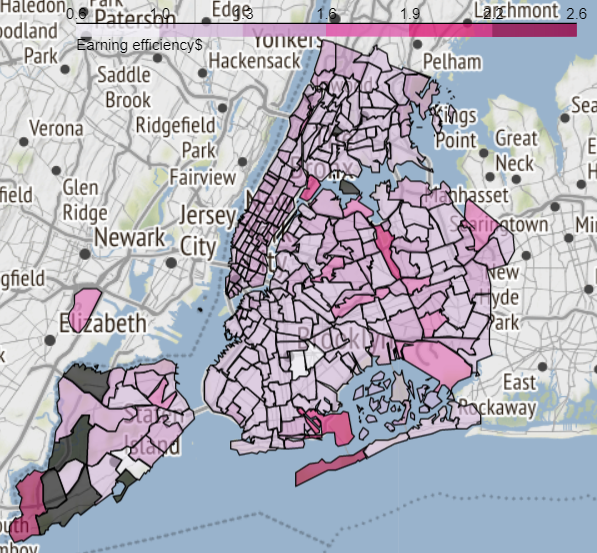
\includegraphics[width=0.95\textwidth]{geo2.jpg}
\end{minipage}
\end{figure}
Figure \ref{f8} shows the log sum of earning efficiency for pick-up location. By taking the sum, both trip amount and the earning efficiency will have weights for the graph, while by taking a log transformation, the weights for the trip amount will not be overstated. As a result, All Manhattan city got a high log sum of earning efficiency, location around the south of Manhattan also gets better performance than the other region. This may be caused by the rules that green taxis cannot pick up in the south part of Manhattan. JFK airport is also a place with good results.

Unlike Figure\ref{f8}, Figure\ref{f9} directly shows the relationship between pick-up location ID and the earning efficiency, although the part with the highest earning efficiency does not appear to be the same as Figure 8, it still provides strong evidence for the relationship between these two features.

\section{Modelling}
The model I choose to use is the Ordinary Least Squares linear regression model(OLS). I decide to use the full model to compare with the reduced model to see whether each feature is related to the response variable and how strong the relationship is.
\subsection{Assumptions}
The assumptions of the linear regression contain: 
\begin{itemize}
\item There is a linear relationship between response and explanatory variable.
\item All the explanatory variables are independent of each other.
\item The residuals follow a normal distribution and have equal variance.
\end{itemize}
For the first assumption, the relationship between the only numerical variable log trip distance with earning efficiency is shown in Figure \ref{f3}, I assumed that there is a certain linear relationship. Moreover, the categorical variables will never break the assumptions for the linear model. For the second assumption, considering the features we have, I think it is pretty fair to assume they are independent of each other. While for the last assumption I have plotted the Q-Q plot(Figure \ref{f10}) and the residual vs fitted value(Figure \ref{f11}) for the full model. Although it has some small outliers in both tails, the Q-Q plot still seems to be fine. On the other hand, the residuals are around zero, and there might be some small variation with the residuals. However, I think it is still fair the assume equal variance.
\begin{figure}[h]
\begin{minipage}{.5\textwidth}
    \centering
    \caption{Q-Q plot}\label{f10}
    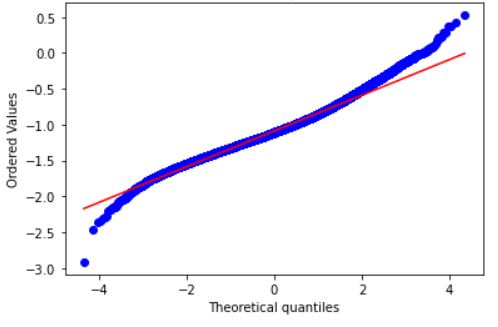
\includegraphics[width=0.95\textwidth]{qq.jpg}
\end{minipage}
\begin{minipage}{.5\textwidth}
    \centering
    \caption{residual vs fitter} \label{f11}
    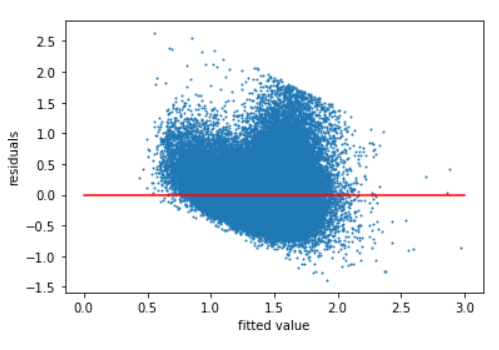
\includegraphics[width=0.95\textwidth]{resfit.jpg}
\end{minipage}
\end{figure}

\subsection{Model Analysis}
I've selected 3 models for contrast: full model, reduced model without snow attribute, and reduced model without log trip distance. The AIC of the full model is 78,710, while the second and the third model got 78,730 and 101,900 AIC. By the comparison of the AIC result, the snow attribute could only have a pretty small influence on the earning efficiency, while the log trip distance would sure have a relatively strong linear relationship with the earning efficiency. Note that the other categorical variables are pretty sure to have a relationship with the response variable in the data analysis part.

After the comparison, now we should focus on the full model. The R-squared is 0.286 which is pretty small to predict the data. However, this is not the research goal of this report. The coefficients of categorical variables pretty much fit the analysis we have made before, which supports the analysis we made. While the coefficient of log trip distance is negative, which means the longer trip distance tends to cause lower earning efficiency.

\section{Recommendations}
After all the analysis, 4 recommendations according to each final feature analyzed(except snow) are suggested for the yellow taxi driver:
\begin{itemize}
\item If taxi drivers can choose the trip on their app, the trip with a shorter trip distance is recommended to choose.
\item Regions in or nearby Manhattan is pretty recommended to start to pick up the passengers, as well as the JFK airport. Try to work around these places.
\item Try not to miss the rush hour(that is, 4 pm to 8 pm ) each day, the trip during these times is considered to have higher earning efficiency. Moreover, due to the trip amount analysis, the waiting time between each trip should be shorter.
\item If you need to rest weekly, try not to miss Monday and Sunday, they turn to have higher earning efficiency for each trip.

\end{itemize}

\section{Discussion}
In conclusion, after analyzing the data, the report has found some useful features that influence earning efficiency and gives suggestions to the yellow taxi drivers. However, by the result of the R-squared, the proportion of earning efficiency gets explained is not pretty high. In order to improve the analysis, I suggest finding more relevant external data sets to find more reasonable features.


\clearpage

% BEGIN REFERENCES SECTION
\printbibliography

\end{document}